\chapter{Methods\label{chap:Methods}}

\section{The \ac{pn/nc} corpus}
Stimuli for the experiments described here were recordings of the \ac{ieee} “Harvard” sentences \citep{HarvardSents} drawn from the \ac{pn/nc} corpus \citep{xxx}.  The 180 sentences in the \ac{pn/nc} corpus were selected from among the 720 \ac{ieee} sentences based on absence of alliteration or rhyming, avoidance of focus/contrast readings, and lack of marked locutions.  The full list of sentences used is given in Appendix~\ref{apx:HarvardSents}.  

Based on within-dialect intelligibility scores from \citet{McCloyEtAl2013}, three talkers were chosen for the present experiments, herein referred to as talkers \ac{a}, \ac{b}, and \ac{c}.  These talkers were selected from among the Pacific Northwest male talkers because, as a group, the Pacific Northwest male talkers exhibited the largest spread in intelligibility in the corpus, and those three talkers formed the endpoints and midpoint of that group, with talker \ac{a} being the most intelligible and talker \ac{c} the least intelligible (cf. Figure~\ref{fig:dotchart}).

\begin{figure}
	\begin{centering}
	\includegraphics{figures/intelDotchart/intelDotchart.eps}
	\caption[Intelligibility of talkers used to make the stimuli]{By-talker mean keywords correct (across 15 dialect-matched listeners) in speech-shaped noise at +2 dB \ac{snr} (data from \citealt{McCloyEtAl2013}).  The three talkers selected for use in the present experiments are indicated by red arrows.\label{fig:dotchart}}
	\end{centering}
\end{figure}

\section{Stimulus creation\label{sec:StimDesign}}
Resynthesized stimuli underwent prosodic replacement, using the \psola{} algorithm as implemented in Praat \citep{praat}.  In all cases, the sentential content of the target file and prosodic donor file were identical (\ie, the contributing recordings were of two different talkers reading the same sentence).  Prosodic replacement requires measurements of intensity and duration for both the target file and the prosodic donor file, as well as information about glottal pulse timing of the target file and pitch contour information from the prosodic donor file.  Methods used to obtain each of these measures is described below.

% Why \psola?  Brief comparison of different methods for manipulating duration.  Malah1979 ("linearly combining adjacent intervals of speech to avoid major discontinuities in the waveform"), MoulinesCharpentier1990 (\ac{psola}).  Relate to the studies that used them: PichenyEtAl1989 (Malah method), UchanskiEtAl1996 (segment-by-segment time scaling), LiuZeng2006 (adding silences, "uniform scaling" = \psola{}?).  Cf KrauseBraida2002, KrauseBraida2004.
% Also one limitation of using \psola{} for resynthesis is the limitation of 50Hz / 20ms

%\subsection{Duration}
Duration measurements for target and donor files were made at the syllable level.  Syllable boundaries were based primarily on local minima in the intensity contour of the sentence.  In cases where intensity contour minima disagreed with phonological syllable affinity, the phonological considerations were given priority.\footnotemark{}  Where intensity contour minima were absent from the syllable transition region, boundaries were marked based on inflection points in the intensity contour or waveform envelope, or in the absence of inflection points, on aspects of waveform or spectrogram morphology.  The segmentation process was aided by a custom Praat script (see Script~\ref{scr:SyllIntens}).

\footnotetext{This arose primarily in cases of fricative-stop onset clusters, where the intensity minimum occured during the stop closure, effectively grouping the fricative into the coda of the preceding syllable.  In such cases, the lack of aspiration on the stop is taken as evidence that it is not in syllable-initial position, and that the syllable boundary should therefore fall before the fricative.}

In order to maximize inter-speaker agreement in number of durational units for a given sentence, the intensity-based syllablewise method of segmentation was chosen over the more common spectrogram-based phonemic\slsh{}allophonic segmentation method \citep[\eg][]{PetersonLehiste1960, TurkEtAl2006}.  For the same reason, the method of marking only periodic\slsh{}aperiodic transitions was also avoided, though otherwise it is particularly well-suited to \psola{} resynthesis.  Whereas there were often inter-speaker disagreements on the number of segments (\eg, eight segments in [pʰɑɹk̚.tʰɹʌk] \vs\ nine in [pʰɑɹkt.tʰɹʌk] for “parked truck”) or the number of periodic\slsh{}aperiodic transitions (\eg, five in [əpʰɑɾətʰi] \vs\ seven in [əpʰɑtəvtʰi] for “a pot of tea”), virtually all sentences in the corpus showed inter-talker agreement on number of syllables.  The rare disagreements were cases of extreme reduction, \eg, sentence 22–07 “It is hard to erase blue or red ink”, in which one talker contracted the initial syllables to “It’s”.  In such extreme cases the sentence was excluded from resynthesis, but in most cases it was still possible to separate the reduced form into two syllable-like units using the same acoustic landmarks mentioned above.  Such sentences were therefore retained to avoid introducing a systematic bias by eliminating the most heavily reduced sentences.

%\subsection{Fundamental frequency}
Fundamental frequency (\fo) information was measured with Praat using a semi-automated process (see Script~\ref{scr:PulseCor}).  For each recording, \fo{} tracks generated by Praat’s pitch tracking algorithm were displayed over a narrowband spectrogram, and algorithm parameters were adjusted as necessary to eliminate spurious pulse detections, pitch halving errors, and other irregularities.  The corrected parameters were then used to create Praat manipulation objects, which allow manual editing of the detected pulses.  After hand-correction of the pulses, sparse \fo{} tracks were re-generated with a single value at the midpoint between each pair of pulses in contiguous voicing regions.

Hand-correction of the pulse points was often necessary in recordings involving creaky voicing, either because the frequency dropped below the algorithm’s pitch floor, or because the amount of jitter\slsh{}shimmer present in the creaky voicing exceeded the level at which the algorithm was willing to mark periodicity (see Figure~\ref{fig:JitShim}a).  In a few such cases, better resynthesis results (as judged auditorily) were achieved by marking each cycle — despite cycle-to-cycle irregularities — rather than omitting alternating pulses in pursuit of a smoother, lower-frequency pitch track (see Figure~\ref{fig:JitShim} for illustration).  %It is speculated that the better resynthesis results arise due to more natural waveform period shapes, allowing the simulation of creaky voicing through \term{pitch wobble}, and the partial undoing of creaky voicing through period regularization.

Prior to being mapped onto the target signal, the locations of donor \fo{} points were shifted via dynamic time warping, with the temporal ratios determined by the relative durations of corresponding syllables in the target and donor files (see Script~\ref{scr:Psola}).  Pitch points were also shifted in frequency so as to equate the mean pitch of the stimulus before and after resynthesis.  This was done to minimize absolute magnitudes of pitch shifts (and thereby minimize distortion due to pitch manipulations), on the assumption that mean \fo{} is irrelevant to the intelligibility of speech (on this point see Section~\ref{sec:IntelPitch}).

\begin{figure}
	\begin{centering}
	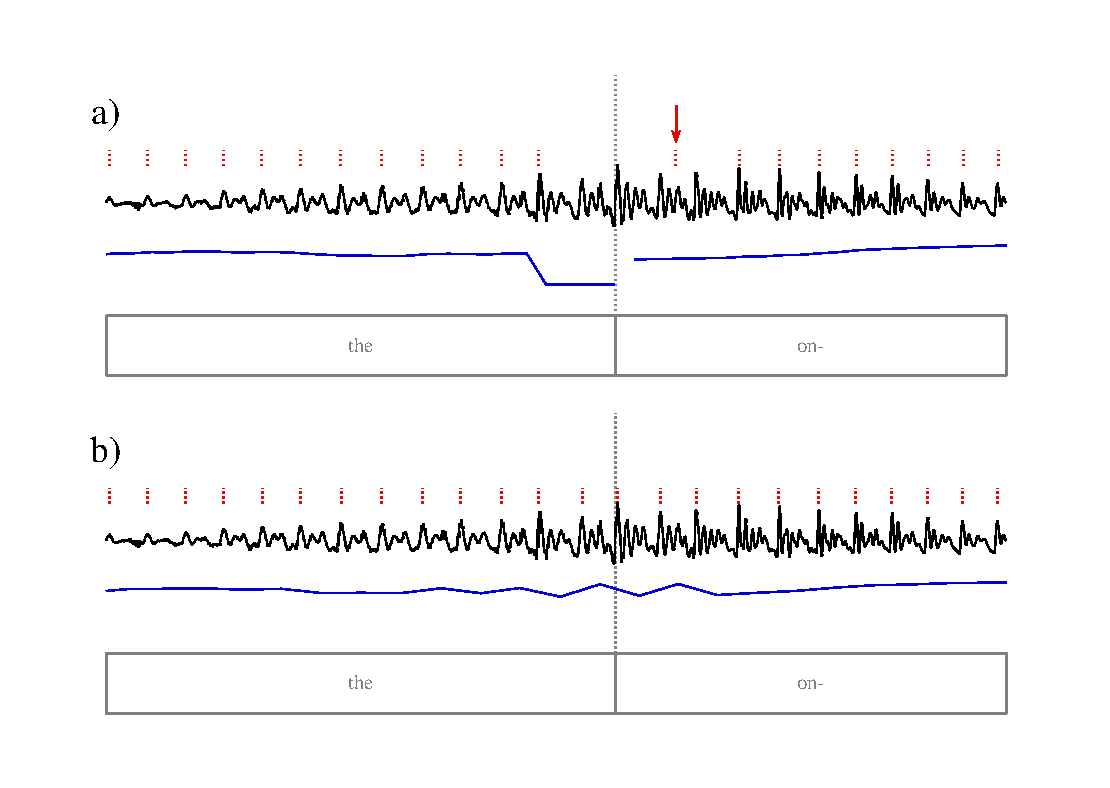
\includegraphics{figures/creakJitterShimmer/creakJitterShimmer.eps}
	\caption[Handling of creaky voicing in resynthesis]{Illustration of method for handling creaky-voiced portions of speech.  (a)~Excerpt of Talker~\ac{b}’s recording of sentence 33–05, in which vowel hiatus is resolved with light creaky voicing.  The waveform (black) is overlaid with Praat’s auto-detected pulse marks (dotted red lines) and pitch track (dashed blue line).  Note the missed cycles on either side of the red arrow, and the phase-shift of all pulses right of the arrow.  (b)~The same span of speech after manual correction of pulses, and a (jittery, but continuous) pitch track generated from the corrected pulses.\label{fig:JitShim}}
	\end{centering}
\end{figure}

%\subsection{Intensity}
Intensity was altered by first multiplying the signal by the difference of the maximum intensity and the inverted intensity contour (see Figure~\ref{fig:IntenManip}), then multiplying the resulting signal by the intensity contour of the replacement prosody and scaling as needed to achieve the desired \ac{rms} amplitude.  To do this, the donor intensity contour first underwent dynamic time warping to match the durational patterns of the target signal (see Script~\ref{scr:Psola}).

\begin{figure}
	\begin{centering}
	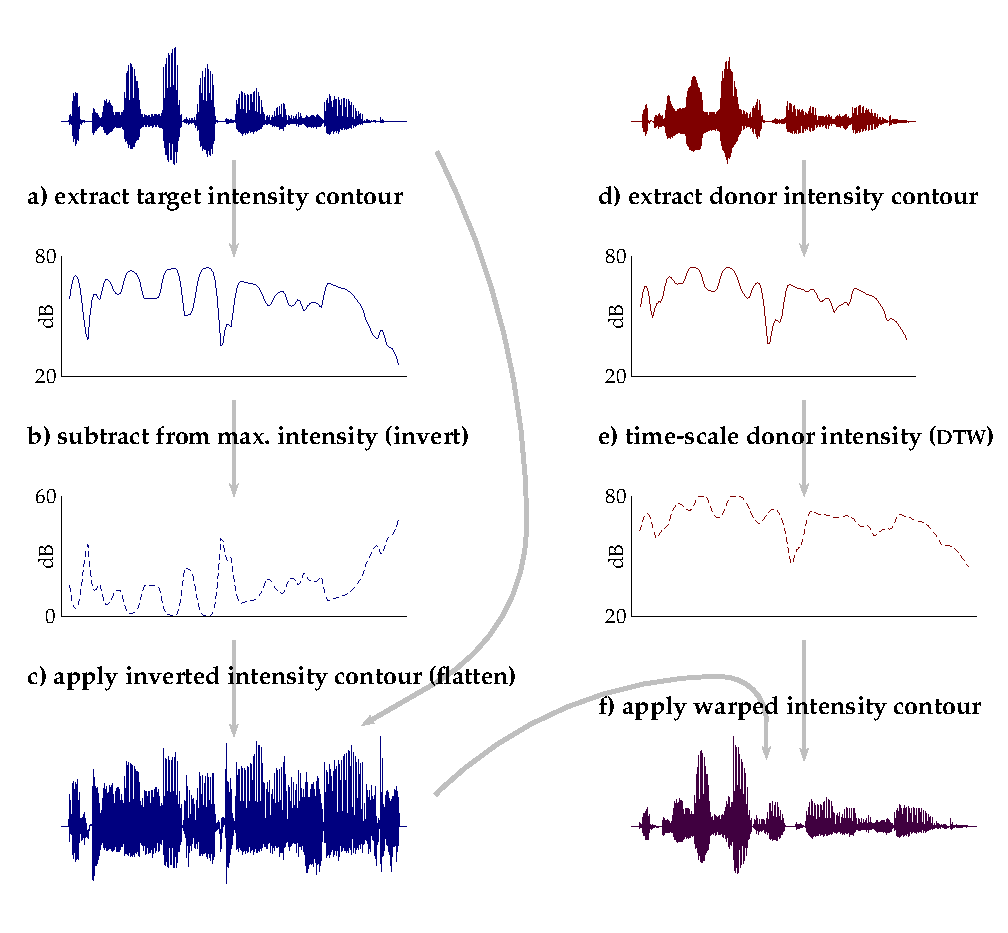
\includegraphics{figures/intensity/intensity2.eps}
	\caption[Intensity scaling in resynthesis]{Illustration of the method used to scale intensity.  (a)~Intensity contour is extracted from target waveform (blue).  (b)~The intensity contour of the target signal is inverted, by subtracting each intensity point from the maximum intensity.  (c)~Target intensity is \term{neutralized} or \term{flattened} by multiplying the target signal by the inverted intensity contour.  (d)~Intensity contour is extracted from the prosodic donor signal (red).  (e)~The prosodic donor intensity contour is time-scaled syllable-by-syllable via dynamic time warping (\ac{dtw}) to match the temporal pattern of the target signal.  (f)~The intensity-neutralized target signal is multiplied by the time-warped donor intensity contour (purple).  The signal is now ready for \psola{} resynthesis of duration and pitch.\label{fig:IntenManip}}
	\end{centering}
\end{figure}

%\subsection{}
After resynthesis, all stimuli were assessed auditorily for excessive distortion.  In some cases, problems could be remedied by readjusting the pulses and pitch tracks and re-running the resynthesis script; in other cases the problems were irremediable, and the unacceptable donor\slsh{}target\slsh{}sentence combination was excluded from the experimental stimuli.  Most cases of irremediable stimuli arose from one of two sources: intra-syllable segment duration and intensity mismatches (see Figure~\ref{fig:SegDurMismatch}), or complete devoicing of a syllable by the target talker (see Figure~\ref{fig:Devoicing}).

\begin{figure}
	\begin{centering}
	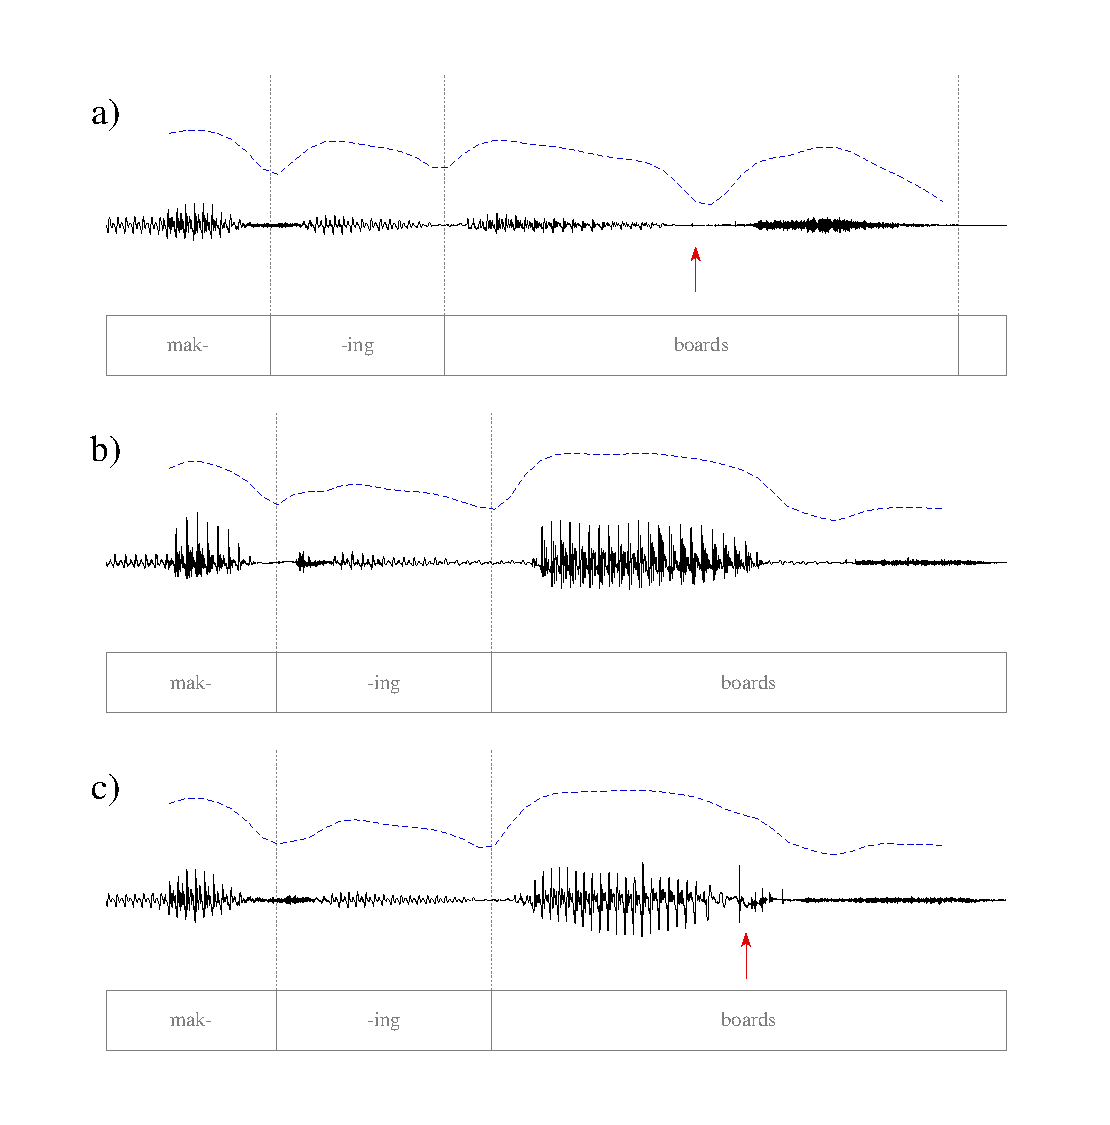
\includegraphics{figures/segmentMismatch/segmentMismatch.eps}
	\caption[Segment duration mismatch in resynthesis]{Illustration of intra-syllable segment duration and intensity mismatch, which led to unnatural patterns of intensity after resynthesis.  (a)~Waveform (black line) of Talker~\ac{c}’s pronunciation of “boards” in sentence 06–05, overlaid with intensity contour (blue dashed line).  Note that the syllable duration is split roughly 50/50 between the periodic nucleus and the aperiodic coda.  (b)~Talker~\ac{a}’s recording of the same sentence.  Note the relatively longer vocalic nucleus and relatively shorter coda.  (c)~Talker~\ac{c}’s waveform after resynthesis to match Talker~\ac{a}’s intensity, pitch, and duration.  The red arrow marks a nearly silent portion of Talker~\ac{c}’s speech that was amplified to vowel-like intensity levels.\label{fig:SegDurMismatch}}
	\end{centering}
\end{figure}

\begin{figure}
	\begin{centering}
	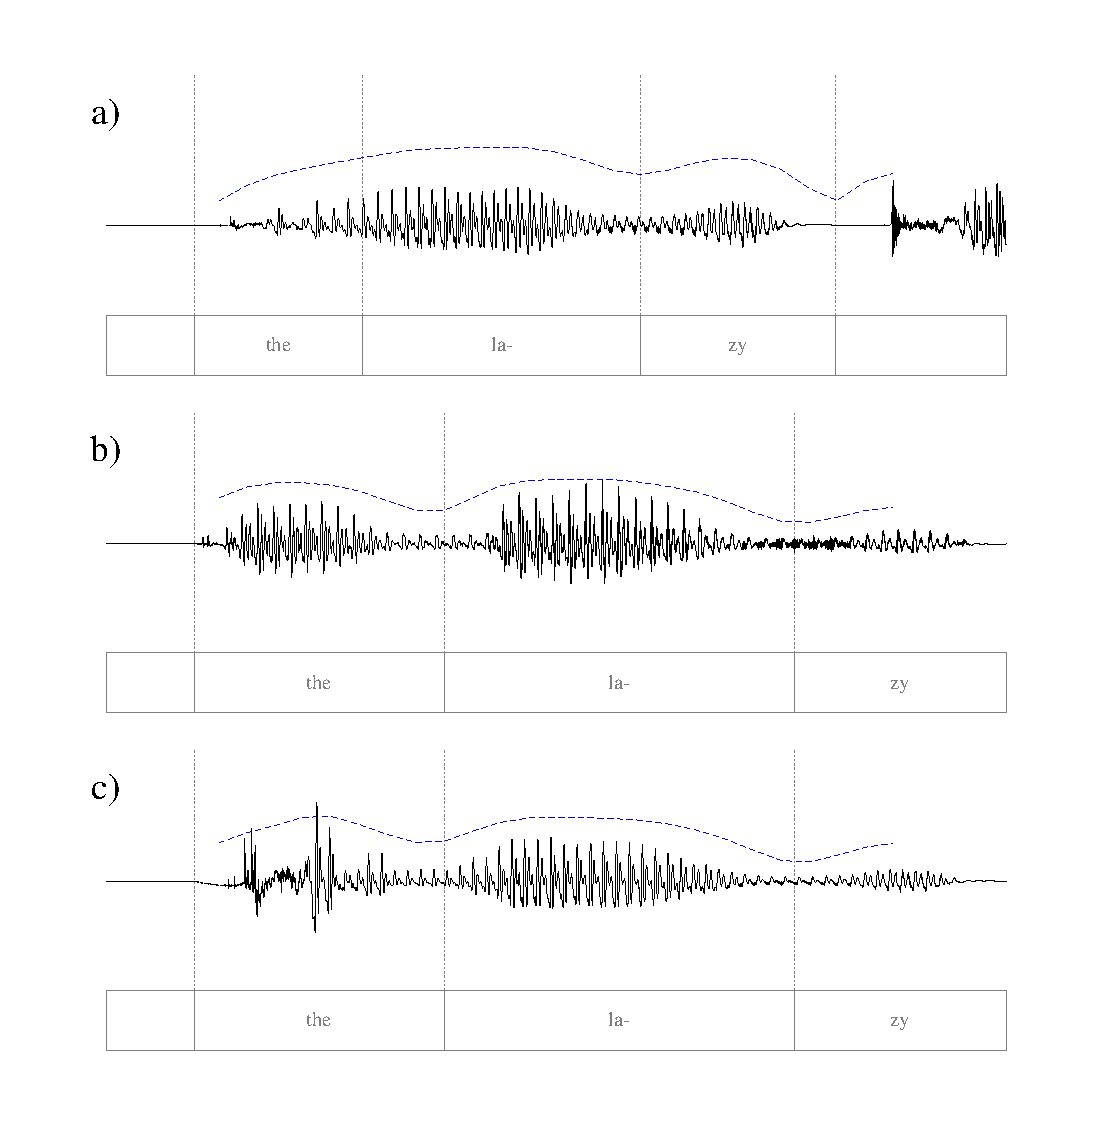
\includegraphics{figures/devoicing/devoicing.eps}
	\caption[Syllable devoicing in resynthesis]{Illustration of how devoicing can lead to unacceptable levels of distortion during resynthesis.  (a) Devoicing of the word “the” in Talker~\ac{b}’s recording of sentence 05–05 (first ≈500 ms shown).  The intensity contour (blue dashed line) is overlaid on the waveform (black).  (b) Talker~\ac{a}’s recording of the same sentence.  (c) Talker~\ac{b}’s waveform after resynthesis to match Talker~\ac{a}’s intensity, pitch, and duration.  Note the excessively high amplitude in the first syllable.\label{fig:Devoicing}}
	\end{centering}
\end{figure}

\section{Experiment sessions}
% Rationale for how much training to do:  
% \citep{YonanSommers2000}: Trained talkerID on 4 talkers (2M2F) over 2 days.  Each day: 60 exposure trials, 40 trials training w/ feedback, 60 more exp, 40 more training, 80 test.  All phases were half high-context and half low-context sentences.  End of day 2: single words \& sentences in SNR -5,0,+5, half high- half low-context, half familiar talkers half novel, half male talkers half female.  Familiar/unfamiliar talkers were piloted to make sure they were equally intelligible generally, and to old vs young people.  RESULTS: young listeners near ceiling on talkerID both day1 and day2; old listeners 73\% and 76\%.  Training on sentence material did not aid on the single word task (same as NygaardPisoni1998).  There was a benefit of familiar talker for sentence materials, which was stronger at lower SNRs.  A similar pattern obtained for a second experiment with talker exposure instead of talkerID training.
% \citep{VanEngen2012}: Two 30-minute training sessions (64 sentences) with noise (either SSN, English 2-babble, Mandarin 2-babble) and feedback.  Posttest 1 familiar, 1 unfamiliar talker, half in English babble, half in mandarin.  Trained and tested at their HINT threshold -3dB (based on VanEngen2010) to avoid floor/ceiling.  Results: “(1) listeners were able to take advantage of target talker familiarity; (2) training with babble was more effective than SSN training; and (3) after babble training, listeners improved most in coping with the babble in which they were trained [English or Mandarin]. In general, the results show that processes related both to tuning in to speech targets and tuning out speech maskers can be improved with auditory training”

Except where otherwise noted, stimuli were presented with a stationary Gaussian masker noise, frequency shaped to match the long term spectral average of the corpus of stimuli, at 0 dB \ac{snr}.  This \ac{snr} was chosen to avoid ceiling and floor effects, based on a pilot study testing five \ac{snr}s ranging from −1 to +3 dB.  To ensure target audibility, the level of the speech was held constant at 67 dB \ac{spl} (dB \ac{rms} in a 6 cc coupler) and the masker noise was digitally added to the speech to achieve the desired \ac{snr}, yielding a final presentation level of approximately 70 dB \ac{spl}.  The noise extended past the beginning and end of the speech by 50 ms in each direction, and linear onset and offset ramps were applied to this excess noise to prevent clicks during stimulus playback.

The combined speech-and-noise signal was presented in a sound-insulated booth over closed-back supra-aural headphones (Sennheiser HD 25–1 II).  Listeners were instructed to repeat each sentence they heard, to give partial answers when they only heard some words, and to guess when they were unsure.  Trials were scored 0–5 on keywords correct during the task.  An audio recording was made of listener responses, and scoring uncertainties were resolved offline.  

Of the 180 sentences in the corpus, half were set aside for use as training\slsh{}exposure sentences in Experiment~2; the remaining 90 sentences were designated as test sentences and resythesized versions of those sentences were created.  Experiment~1 presented the 90 test sentences to each listener, with equal numbers of stimuli from each “talker” (\ie, ten from each of the three unmodified talkers \ac{a}, \ac{b}, and \ac{c}, plus ten from each of the six resynthesized “talkers” \ac{ab}, \ac{ac}, \ac{ba}, \ac{bc}, \ac{ca}, and \ac{cb}).  Talker-sentence combinations were random and unique for each listener, subject to the above-mentioned constraints (\ie, each listener heard each talker an equal number of times, and each listener heard each sentence only once).

In Experiment~2, the 90 training sentences were presented in speech-shaped noise at 0 dB \ac{snr}.  After each listener had finished responding, the sentence was played again without background noise, and the text of the sentence was simultaneously presented on a computer screen for the listener to read.  For a given listener, all 90 training sentences were recordings of the same talker, but the test sentences were again drawn in equal numbers from among the three unmodified talkers (\ac{a}, \ac{b}, and \ac{c}) and the six resynthesized “talkers” (\ac{ab}, \ac{ac}, \ac{ba}, \ac{bc}, \ac{ca}, and \ac{cb}).

This design of the training phase — to include stimuli both with and without noise maskers — was chosen for several reasons.  First, stimuli with noise were included to maximize similarity between the training and testing phases, and also to first expose listeners to only the speech cues that are sufficiently robust to escape from the masker.  At the same time, auditory feedback presented without a noise masker was included so that listeners had access to all possible speech cues during training, to provide both reinforcement of the robust speech cues and additional complementary information that would (hopefully) facilitate the process of talker familiarization.

\section{Scoring\label{sec:Scoring}}
Each trial was scored 0–5 based on number of keywords correct.  Keywords were all content words, though a few sentences included pronouns among the keywords.  This likely added some variability in the difficulty of sentences, since pronominal forms are more likely to undergo reduction in speech, and are often highly confusible (\eg, \term{him} \vs\ \term{them}).  However, differences in difficulty from sentence to sentence were unavoidable in any case, since across sentences the keywords varied in their lexical frequency and their predictability from sentential context.  Both of these shortcomings of the stimuli are overcome by explicitly including variability in sentence difficulty as part of the statistical model (see Section~\ref{sec:DataAnal}).

Another potential problem with scoring based on keywords is that discrete scores from 0 to 5 are not necessarily well-modeled as a continuous outcome in statistical models.  One solution to this problem is to model the outcome as an ordered multinomial variable, though such models are complicated and difficult to implement computationally.  An alternative solution is to score sentences in an “all-or-nothing” fashion, and model the outcome as a binomial distribution (for which well-tested computational methods exist).  The drawback of binary scoring is that information about partially correct responses is lost, and models are less intuitive to interpret (model coefficients are “logits” instead of keywords correct).

In analysing these experiments, a hybrid approach is taken: both continuous and binomial models are constructed, and as long as the continuous model agrees with the corresponding binomial model in the direction and significance of the predictors, the results of the continuous model are reported to facilitate the interpretation of model results.  This approach comes with the caveat that the absolute magnitudes of the coefficients should be interpreted somewhat cautiously.

\section{Participants}
Listeners were all native English speakers who lived in the Pacific Northwest (Washington, Oregon, or Idaho) throughout their period of primary and secondary education (\ie, ages 6–18).  All reported English as the primary home language, and all had learned or studied at least one other language as an adolescent or adult (though this was not a criterion for inclusion).  All listeners had bilaterally normal hearing, defined as pure-tone thresholds of 20 dB \ac{hl} or better at octave intervals from 250 Hz to 8 kHz \citepalias[re:][]{ansi2004}.  Listeners were recruited from the UW campus community and were compensated for their participation; there were 17 listeners in Experiment~1, and 20 listeners in Experiment~2.  One participant was excluded from Experiment~1 due to a mild monaural threshold elevation at 8 kHz.  Listener demographics are summarized in Table~\ref{tab:ListDemo}.

\begin{table}
	\caption[Listener demographics]{Listener demographics for Experiments~1 and~2.  Experiment~2a represents the listener group trained on Talker~\ac{c}; Experiment~2b represents the listener group trained on a talker not among the test talkers.\label{tab:ListDemo}}
	\centering
	\begin{tabu} to 0.6\textwidth {llX[2]XXX}
		\toprule
		\rowfont{\bfseries} & & & \multicolumn{3}{c}{Experiment}\\
		\rowfont{\bfseries} & & & 1 & 2a & 2b\\
		\midrule
		\textbf{Gender} & Female & & 8 & 0 & 0\\
		                & Male   & & 8 & 0 & 0\\
		\midrule
		\textbf{Age} & mean      & & 22.3 & 0 & 0\\
		             & st.\ dev. & &  6.9 & 0 & 0\\
		             & min.      & & 18   & 0 & 0\\
		             & max.      & & 44   & 0 & 0\\
		\taburulecolor{ltgray}
%		\midrule
%		Ethnicity & & & \\
		\taburulecolor{black}
		\bottomrule
	\end{tabu}
\end{table}

\section{Data analysis\label{sec:DataAnal}}
As mentioned in Section~\ref{sec:ExpDesign}, the contribution of prosody to intelligibility is most easily seen when talkers vary in their base intelligibility, whereas the effect of familiarity is most easily seen when the base intelligibility of the talkers is known to be equal.  Analysis using mixed-effects regression addresses this problem by simultaneously estimating the influence of multiple predictors or \term{fixed effects}, as well as estimating residual within-group variability due to uncontrolled factors or \term{random effects} (\eg, variability in item difficulty or listener ability).  In other words, mixed-effects models can estimate the effect of familiarity {\emph as if} the base intelligibility of the talkers were equal.

In these experiments, the fixed effects are all binary variables or multi-level factors dummy-coded as binary variables, so the estimated coefficients of the linear model represent differences between groups of stimuli.  Data were analyzed using R \citep{R}, with the packages {\inlinecode lme4} for mixed-effects regression \citep{lmer} and {\inlinecode languageR} for Markov-chain Monte Carlo simulation of model parameters \citep{languageR}.

For Experiment~1 (testing the effect of prosodic replacement on intelligibility), the fixed-effect predictors used in the model are {\inlinecode resynth}, {\inlinecode segDonor} and {\inlinecode proDonor}.  {\inlinecode Resynth} is a Boolean variable that is true for Talkers~\ac{ab}, \ac{ac}, \ac{ba}, \ac{bc}, \ac{ca} and~\ac{cb}, and is included as a control for the distortion introduced by the resynthesis process.  {\inlinecode SegDonor} represents the talker used as the base waveform for the resynthesis, and {\inlinecode proDonor} represents the talker whose prosody was used in the resynthesis.  Both {\inlinecode segDonor} and {\inlinecode proDonor} are three-level factors, each recoded into a pair of dummy-coded binary variables for modeling purposes.  For stimuli that were not resynthesized, the value of {\inlinecode segDonor} and {\inlinecode proDonor} are the same.  Random effects are included for both sentence and listener, to account for the fact that not all sentences are equally difficult (cf. Section~\ref{sec:Scoring}), and the fact that listeners are not necessarily equally skilled at speech-in-noise tasks.  A manual “drop-1” procedure using likelihood-ratio tests was used to validate the inclusion of each of the fixed-effects predictors; in all cases, a significantly better model fit was realized with each predictor than without it.

For Experiment~2 (testing the role of prosody in the familiar talker advantage), the fixed-effect predictors include all those used for Experiment~1, plus two additional predictors: {\inlinecode segTrain} is a Boolean variable indicating match between the training talker and the segmental donor of the test stimulus, and {\inlinecode proTrain} likewise indicates a match between the training talker and the prosodic donor of the test stimulus.  As in Experiment~1, random effects are included for both sentence and listener, and a manual “drop-1” procedure confirmed the validity of including each fixed-effect predictor.

\comment{I may say more here when I finalize exactly which post-hoc tests I’m doing.}
